%% bare_jrnl.tex
%% V1.4b
%% 2015/08/26
%% by Michael Shell
%% see http://www.michaelshell.org/
%% for current contact information.
%%
%% This is a skeleton file demonstrating the use of IEEEtran.cls
%% (requires IEEEtran.cls version 1.8b or later) with an IEEE
%% journal paper.

\documentclass[journal,onecolumn]{IEEEtran}
%
% If IEEEtran.cls has not been installed into the LaTeX system files,
% manually specify the path to it like:
% \documentclass[journal]{../sty/IEEEtran}

\usepackage[pdftex]{graphicx}
\usepackage{amsmath,amssymb,amsfonts,amsthm}
\usepackage{algpseudocode}
\usepackage{algorithm}
\usepackage{xpatch}
\usepackage{cite}
\usepackage{tikz}
\usetikzlibrary{shapes, arrows, arrows.meta}

\ifCLASSOPTIONcompsoc
\usepackage[caption=false, font=normalsize, labelfont=sf, textfont=sf]{subfig}
\else
\usepackage[caption=false, font=footnotesize]{subfig}
\fi

\newtheorem{lemma}{Lemma}
\renewcommand{\IEEEQED}{\IEEEQEDclosed}

%\usepackage{array}
%\usepackage[caption=false,font=normalsize,labelfont=sf,textfont=sf]{subfig}
\usepackage{url}

\hyphenation{}

%% For algorithms...
\algnewcommand\algorithmicforeach{\textbf{for each}}
\algdef{S}[FOR]{ForEach}[1]{\algorithmicforeach\ #1\ \algorithmicdo}
\algnewcommand\algorithmicswitch{\textbf{switch}}
\algnewcommand\algorithmiccase{\textbf{case}}
\algdef{SE}[SWITCH]{Switch}{EndSwitch}[1]{\algorithmicswitch\ #1\ \algorithmicdo}{\algorithmicend\ \algorithmicswitch}%
\algdef{SE}[CASE]{Case}{EndCase}[1]{\algorithmiccase\ #1}{\algorithmicend\ \algorithmiccase}%
\algtext*{EndSwitch}%
\algtext*{EndCase}%

\begin{document}
% \title{_}
% \author{_}
% 
% \maketitle

\section{Introduction}
The use of spatial data structures is ubiquitous in many areas ranging from computational geometry, robotics and geographic information systems.  It has important advantages to offer to current spatial algorithms in particular the application of spatial indexes and opportunities to exploit proximity among the data.  Many works depends on it to ensure efficiency for example spatial joins, voronio diagrams and robot motion planning \cite{berg_computational_2008}.

Although spatial data structure such as grids and the different flavours of rtrees and quadtrees are widely reported in literature, other structures have been less the focus of attention.  In particular, edge-list structures appear as a technique used in diverse applications, specially related with geometric computation, but their employment have been limited to very specific domains.  The use of such kind of structures has been reported in applications like obtaining silhouettes of polyhedra, efficient Minkowksi sums and offset of polygons and diverse types of triangulations mainly in computational geometry projects.

The most representative data structure in the edge-list family is the Double Connected Edge List (DCEL).  A DCEL \cite{muller_finding_1978, preparata_computational_1985} is a data structure which collect topological information of the edges, vertices and faces contained by a surface in the plane.  The DCEL and its components represent a planar subdivision of that surface in the plane. In a DCEL, the faces (polygons) represents the cells of the subdivision; the edges are boundaries which divide adjacent faces; and the vertices, itself, are boundaries between adjacent edges.

One interesting problem in which edge-list data structures have shown utility are the thematic overlay maps. In this problem, two polygon input layers capture geospatial information and attribute data for different kind of phenomena.  In many areas, such as ecology, economics and climate change, it is important to be able of join those layers and match their attributes in order to unveil patterns or anomalies in data which can be highly impacted by location.  Several operations are relevant depending of the study, for instance, sometime the user would like to find intersections between the layers and other times be able to see the difference between them. 

Even the DCEL data structure has interesting advantages for overlay map operations, current methods are sequential based.  For layers with thousand of polygons the execution time is not feasible.  Further more, most of distributed techniques that have been used in this matter are oriented to a specific spatial operation (intersection, union or difference) and they have to be run from scratch if other operation is required.  In addition, current parallel techniques divide the data into partitions and replicate features if needed in order to solve the problem locally.  It could potentially increase the size of the problem.  Up to now, data structures collecting topological properties, like the DCEL, are not explored in a distributed and scalable fashion in order to support typical overlay operators.

Even sequential DCEL implementation are not new, nowadays, with the scale and volume of available geodata, the rise of big (spatial) data makes necessary to count with fast and efficient techniques for spatial analysis.  For example, today GIS researchers have to deal with spatial operations between layers collecting thousand of counties boundaries at nation-wide level.  The versatility and efficiency of the spatial methods is cardinal for their studies. Given the advantages shown by the DCEL data structure, it should be interesting to count with intermediate data structures that not just exploit the advantages of distributed frameworks but also allow multiple map overlay queries at the same time. 

In addition, we already know that current topological data structures are common in computational geometry.  However, most implementations are sequential and they do not scale appropriately on large spatial datasets.  Moreover, distribute alternatives like parallel spatial joins add complexity due to spatial partitioning and replication and they are unable to run more than one operation once they have been created.

In this paper we describe the design and implementation of a scalable and distributed DCEL data structure.  To do that, we face some important challenges.  First, a partition strategy that ensure a correct split of the input data needs to be presented.  It should guaranteed that each partition collect the required data to work independently minimizing duplication and transmission costs.  In addition, the partition strategy must present a merging procedure that guarantee the collection of all the individual results and the consolidation of the final and correct answer.

Secondly, the proposal must be ready to deal with potential anomalies which are not present in sequential execution.  For example, the implementation should apply appropriate management of features such as holes and multi-polygons which could lay on different partitions.  Such features could potentially lost the reference of their other components compromising the correctness of the implementation.  Appropriate mechanism should be applied to solve these possible problems.

Finally, once a scalable and distributed DCEL has been built, it must support a set of Boolean overlay operations in a transparent manner.  It is, the query of such operators should take advantage of the scalability of the DCEL and be able to run also in a parallel fashion.  Additionally, the different operators should be able to be run multiple times without the need of rebuild the data structure.  So, the pertinent adjusts to the overlay operations should be addressed as well.

The contributions of this work contribute to the solution of the above-mentioned challenges.  We present and discuss the implementation of a novel strategy to divide the input data and build a distribute and scalable DCEL to be used in a parallel framework such as Apache Spark.  We address the complexities that such partitioning schema could arise and provide Boolean overlay operation that work efficiently on top of our scalable DCEL data structure.

At the best of our knowledge, there is not a distributed and scalable DCEL implementation available that meet those criteria.  We think it could be a great tool to support key  challenges and operations in Geoscience today.
\newpage
\section{Literature review}
The fundamentals of the DCEL are explained in the seminal paper of \cite{muller_finding_1978} and illustrated with more examples in \cite{preparata_computational_1985}.  The authors highlight among the main advantages of DCELs the opportunity of capturing topological information and allowing multiple overlay operations once the DCEL is created.  In addition, a DCEL can be constructed in $\mathcal{O}(n log(n))$ time using $\mathcal{O}(n)$ additional memory where $n$ is the number of vertices in the input layer \cite{freiseisen_colored_1998}. Once created, the DCEL allows Boolean overlay operations in $\mathcal{O}(n)$ time using $\mathcal{O}(n)$ additional space. 

Nowadays, implementations of DCEL data structures have been presented and used in diverse applications.  \cite{barequet_dcel_1998} presented the description and modelling of a database-oriented implementation of a DCEL. It presents a geometric package aims to support polyhedra or polyhedral surface operations.  The design is discussed in detail together with application examples for collision detection, gap filling and inter-slice interpolation.

In \cite{freiseisen_colored_1998}, the author explains in more detail the different spatial operations (intersection, union and difference) supported by a DCEL while describes a sequential implementation over the Computational Geometry Algorithms Library - CGAL.  This work allows, given two simple polygon layers, the intersections of their boundaries keeping track of related attributes of the inputs.  

A cardinal reference for DCEL description and design should be \cite{berg_computational_2008}.  It describes the core of the DCEL construction algorithm but also go deeper in the explanation of related concepts and techniques used during the DCEL generation such as line segment intersection and plane sweeping methods.  It also compiles a number of well-explained examples and applications of its usage, for instance, triangulations, point location and robot motion planning.

\cite{boltcheva_topological-based_2020} describes the use of sequential DCELs to store the needed topological information of mesh networks extracted from LiDAR data to reconstruct roof polygons in 2D.  They highlight the usefulness of 2D topological data structures to avoid the complexities in data storage and handling of 3D configurations.

Although there is not reference to distributed DCEL implementations, other dynamic parallel data structures has been described.  For example, the DD-Rtree \cite{challa_dd-rtree_2016} claims to preserve spatial locality while distributing data across compute nodes.  By contrast to static counterparts, it can be constructed incrementally making it useful for handling big data.  It evaluates its communication cost, query time and data performance of data mining algorithms.  In addition, this work provides an interesting survey of multi-dimensional indexing structures and their parallel versions.  Similarly, \cite{sabek_spatial_2017} describe different techniques to support distributed spatial joins, including options to perform spatial partitions in layers previous to the join phase.  Together with this, it evaluates cost-based and rule-based query optimization.  

However, spatial indexes and spatial joins could support overlay operations in certain way but just for an individual operator at a time. 

\cite{li_scalable_2019} also explore parallel support for common computational geometry operations including polygon union, convex hull and skylines.  They apply the MapReduce paradigm over the Hadoop framework presenting the CG\_Hadoop tool.  However, as before, it just supports limited number of operations over an individual input layer once at a time.

\cite{franklin_data_2018} also present a survey of parallel spatial algorithms but it focus on GPU and multi-core architecture.  They mention works related to hierarchical tree structures (octree or rtree), location point algorithms, line and plane sweep algorithm, cluster-based parallel map overlays, among others.  Also, they mention the use of those techniques in the solution of diverse operations such as: union of large set of polygons, planar graphs, overlaying maps, 3D overlay triangulation and cross areas in overlay polygons.

\cite{magalhaes_fast_2015} performs the map overlay in parallel, thereby utilizing the ubiquitous multi-core architecture.  It uses a two-level grid partitioning strategy and proposed a conservative empirical formula for the grid size that gave a good execution time and a feasible memory size.  Together with this, they implement exact computation using rational number to overcome round-off errors. As result, they provide the EPUG-Overlay package to support intersection operations.

\cite{puri_efficient_2013} and \cite{puri_mapreduce_2013} revisit the distributed polygon overlay problem and its implementation using the GPGPU model and the MapReduce paradigm respectively.  \cite{puri_mapreduce_2013} present the adaptation and implementation of a polygon overlay algorithm and describe the system to execute a distributed version on a Linux cluster using Hadoop MapReduce framework.  However, they only analyze and report intersection overlay operation since it is the most widely used and representative operation.  They ported an MPI based spatial overlay system (GPC library) to Hadoop MapReduce platform and a grid based overlay algorithm with two alternatives: a single map and reduce phase, and a map phase only using distributed caches.

In \cite{puri_efficient_2013}, the research focuses to develop an array based parallel overlay algorithm which can be easily implemented on GPUs using prefix sum and sorting to,  potentially, speedup overlay computation.  In this approach, they use a distributed Rtree construction using a top-down schema and a load-balanced overlay processing system using the MapReduce paradigm.  The proposed parallel algorithm uses a similar idea of a DCEL with the representation of a new set of polygons by the merge of edges from the initial layers and their intersections.  However it uses scan lines to partition the set of edges and process them concurrently. As the previous work, they test the implementation only with the intersection overlay operation.

Theses previous works focus on solutions aim to multi-core architectures or GPGPU models which scalability can be affected by very large datasets.  Even though, implementations over the Hadoop ecosystem could not take total advantage of modern distributed memory frameworks such as Apache Spark.

Currently, there are just a few sequential implementations available in the market.  The most important are LEDA\footnote{\url{https://www.algorithmic-solutions.com/}} \cite{mehlhorn_leda_1995}, Holmes3D\footnote{\url{http://www.holmes3d.net/graphics/}} \cite{holmes_dcel_2021} and CGAL\footnote{\url{https://www.cgal.org/}} \cite{fogel_cgal_2012}.  LEDA and Holmes3D are close-source software and their access is limited.  On the other hand, CGAL is an open-source project with a large trajectory in the area of computational geometry offering a wide-ranging number of packages and modules to support diverse areas from modular arithmetic to geometric optimization.

CGAL offers a solid support for DCEL construction and overlay operations on top of it through the Arrangement package.  Its design concepts, implementation and well documented applications are available by different sources (\cite{flato_design_2001}, \cite{haran_experimental_2009} and \cite{wein_advanced_2007}).  \cite{fogel_cgal_2012} deserves a particular entry.  It does just not demonstrate the features of the DCEL implementation but also it collects a large number of application in diverse and novel areas like computer-assisted surgery and molecular biology.

\newpage
\section{Methods} \label{sec:methods}

\subsection{Preliminaries}
There are some useful concepts to keep in mind in order to understand the creation and use of a DCEL data structure.  It starts with a set of edges, pair of two vertices, start and end, which define its orientation. We assume every edge is an straight line segment.

Define edge
Define half-edge: An edge usually bounds two faces, so we need two pairs of pointers for it. It is convenient to view the different sides of an edge as two distinct half-edges, so that we have a unique next half-edge and previous half-edge for every half-edge. This also means that a half-edge bounds only one face. The two half-edges we get for a given edge are called twins. (paraphrase)
Define Face: a face is a polygonal region whose boundary is formed by connected edges and vertices.  The main idea is that the faces of the resulting DCEL can be able to reconstruct the original polygons.

State the problem
The current challenge is the construction of a distributed and scalable DCEL structure that allows the querying of overlay operations, such as intersection and difference, over a large set of polygons.

Overview of the solution
The main idea of the solution is to partition the edges from each of the polygons using a spatial data structure (for instance, a quadtree).  Edges contained at each section of the partitioning will be the input of a local DCEL which will store the information of the vertices, half-edges and faces for their edges clipped to the boundary of its spatial partition.  Each local DCEL can be seen as an individual structure which can be queried and the solution will be later merged with the other local DCELs to complete the final answer. 

\subsection{Partition strategy} \label{sec:strategy}
In many cases, the operations provide by a DCEL could involve large spatial datasets.  Our aim is to offer a solution to deal with data volumes that the current sequential solution are unable to process.  In order to reach that goal we are purposing a partition strategy to build a scalable DCEL in a parallel fashion.  

The main idea of the strategy is to split the study area into a number of cells which could be processed independently in a local basis. We can take the case of overlay operations over layers of polygons as an example to explains the details. In the sequential approach, the DCEL for each layer will be built and then both will be merged to generate a structure where the operator can be applied.  

Our goal is to create DCELs for each layer in parallel to be able to solve large datasets the sequential alternatives are unable.  The proposal can be summarized in the following steps: (i) Partition the input polygons and build local DCEL representations of them at each partition; (ii) Merge the local DCELs for each layer together locally scaling the processing cost; (iii) Overlay operations will be run over the local merged DCELs to finally be collected back to mix and generate the final answer.  

The proposed partition schema is illustrated in figure \ref{fig:overlay_parted}.  First, we will use a sample of edges from both layers to create a set of cells which will spatially partition the space into disjoint areas.  In the example, a simple grid is used but any spatial index can be applied (in our experiments we use quadtrees for better balance and data distribution).  We will use those cells to clip the input polygons to generate new ones that will lie inside of the boundaries of the cell.  Although it will increase the number of edges and the size of the data, we expect that that the gain during parallel processing will make the addition worthwhile.

\begin{figure*}[!ht]
    \centering
    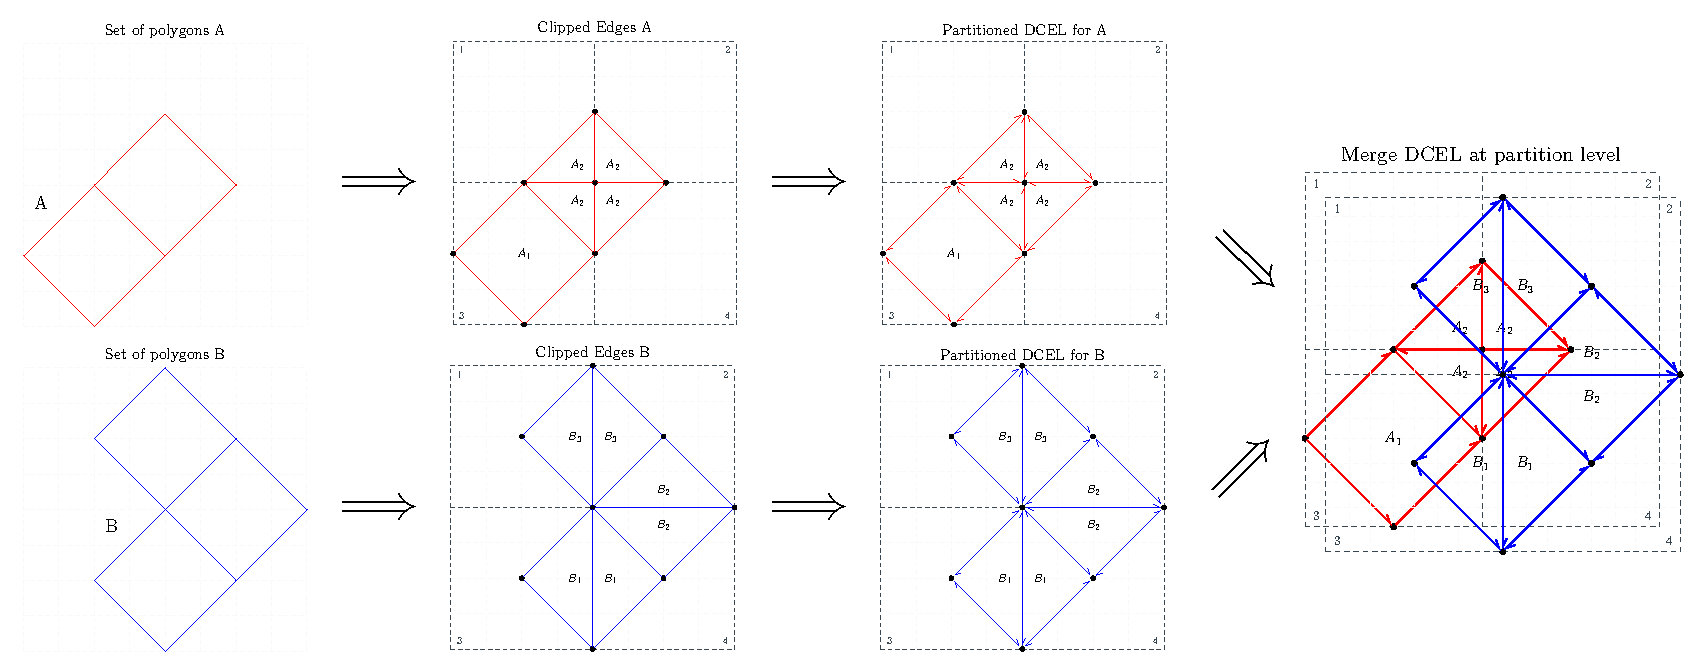
\includegraphics[width=\textwidth]{figures/01-OverlayParted}
    \caption{Partition schema.}\label{fig:overlay_parted}
\end{figure*}

Now each cell have the enough data to build a DCEL representation of the new polygons for each layer.  Data for each cell will be marked appropriately and submitted to different nodes to be processed in parallel.  Note that the same partition schema (set of cells) is used in both layers.  That is important due to it allows one-to-one matching between corresponding partitions in both layers.

During the local DCEL construction for individual layers, it is straightforward the connection between the edges inside of each polygon.  From the inputs, it can easily be identified the position of each edge relate to its next and previous edges and to which face's (polygon's) boundary the edge belongs.  Each edge is converted to a half-edge and their pointers are update accordingly.  However, a query to identify the twin pointer of each half-edge is still needed given that the input polygons do not provide which polygons are in its neighborhood. The matching is done through a self-join query among the current half-edges to pair those which share the same vertices in opposite directions.

However, when we pair the partitions from the both layers, we got two local DCELs (each representing the polygons for each layer) and the processing we need now is a merge between both of them.  It requires: (i) Identify the intersection points between the half-edges of each local DCEL and add them as new vertices; (ii) Split those half-edges involve in an intersection with a recently added vertex (prune duplicates if needed); (iii) Traverse the list of vertices and update their incident half-edge list; (iv) Update the pointers for next and previous half-edges in those affected by the splits; (v) Update the list of faces and their corresponding labels.

Figure \ref{fig:part2} depicts an overview of the process taking as example the polygons and edges of partition 2 of figure \ref{fig:overlay_parted}.  Similarly, figure \ref{fig:merged_dcel} shows the full result of the merged DCEL once all the partitions have processed their corresponding edges. Note that red half-edges have been introduced artificially by the partition schema but they are marked accordingly to be used in the collect back process when we need to unify the results after the application of the overlay operations.

\begin{figure}[!ht]
    \centering
    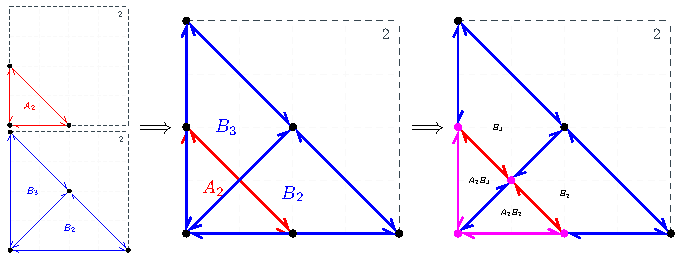
\includegraphics[width=0.9\linewidth]{figures/02-Part2}
    \caption{Merge of local DCEL for partition 2.}\label{fig:part2}
\end{figure}

\begin{figure}[!ht]
    \centering
    \tikzset{    
    barbarrow/.style={ % style that just defines the arrow tip
        %>={Straight Barb[left,length=5pt,width=5pt]},
        >={Triangle[left,length=5pt,width=5pt]},
        double,
        semithick,
        <->
    },
    whites/.style={
        thick, 
        color=white
    }
}
\definecolor{light-gray}{gray}{0.9}
\scalebox{0.9}{
\begin{tikzpicture}
    \tikzstyle{node1}=[draw,scale=0.4,shape=circle,color=black,fill=black]
    \tikzstyle{node2}=[draw,scale=0.4,shape=circle,color=red,fill=red]    
    \draw[color=light-gray, style=dashed] (0,0) grid (8,8);
    \draw[color=red, style=dashed, step=4] (0,0) grid (8,8);
    \node[node1] (A) at (0,2) {};    \node[node1] (C) at (2,0) {};
    \node[node1] (D) at (2,2) {};    \node[node1] (E) at (2,4) {};
    \node[node1] (F) at (2,6) {};    \node[node1] (G) at (3,1) {};
    \node[node1] (H) at (3,3) {};    \node[node1] (I) at (3,5) {};
    \node[node1] (J) at (4,0) {};    \node[node1] (K) at (4,2) {};
    \node[node1] (L) at (4,4) {};    \node[node1] (M) at (4,6) {};
    \node[node1] (N) at (4,8) {};    \node[node1] (O) at (5,3) {};
    \node[node1] (P) at (5,5) {};    \node[node1] (Q) at (6,2) {};
    \node[node1] (R) at (6,4) {};    \node[node1] (S) at (6,6) {};
    \node[node1] (T) at (8,4) {};

    \node at (1,2)      {$A_1$};
    \node at (6.5,4.6)  {$B_2$};
    \node at (6.5,3.4)  {$B_2$};
    \node at (3.4,6.5)  {$B_3$};
    \node at (4.6,6.5)  {$B_3$};
    \node at (4.6,1.5)  {$B_1$};
    \node at (3.6,1)    {$B_1$};
    \node at (3,4.4)    {$A_2$};
    \node at (3,3.6)    {$A_2$};
    \node at (3,2)              {$A_1B_1$};
    \node[scale=0.6] at (3.6,3) {$A_2B_1$};
    \node[scale=0.6] at (4.4,3) {$A_2B_1$};
    \node[scale=0.6] at (5,4.4) {$A_2B_2$};
    \node[scale=0.6] at (5,3.6) {$A_2B_2$};
    \node[scale=0.6] at (3.6,5) {$A_2B_3$};
    \node[scale=0.6] at (4.4,5) {$A_2B_3$};
    
    \draw[barbarrow] (A) -- (C);\draw[barbarrow] (A) -- (E);
    \draw[barbarrow] (C) -- (G);\draw[barbarrow] (D) -- (G);
    \draw[barbarrow] (D) -- (H);\draw[barbarrow] (E) -- (H);
    \draw[barbarrow] (E) -- (I);\draw[barbarrow] (F) -- (I);
    \draw[barbarrow] (F) -- (N);\draw[barbarrow] (G) -- (J);
    \draw[barbarrow] (H) -- (L);\draw[barbarrow] (I) -- (L);
    \draw[barbarrow] (I) -- (M);\draw[barbarrow] (J) -- (Q);
    \draw[barbarrow] (G) -- (K);\draw[barbarrow] (H) -- (K);
    \draw[barbarrow] (K) -- (O);\draw[barbarrow] (L) -- (O);
    \draw[barbarrow] (L) -- (P);\draw[barbarrow] (M) -- (P);
    \draw[barbarrow] (N) -- (S);\draw[barbarrow] (O) -- (Q);
    \draw[barbarrow] (O) -- (R);\draw[barbarrow] (P) -- (R);
    \draw[barbarrow] (P) -- (S);\draw[barbarrow] (Q) -- (T);
    \draw[barbarrow] (S) -- (T);
    
    \draw[whites] (A) -- (C);\draw[whites] (A) -- (E);
    \draw[whites] (C) -- (G);\draw[whites] (D) -- (G);
    \draw[whites] (D) -- (H);\draw[whites] (E) -- (H);
    \draw[whites] (E) -- (I);\draw[whites] (F) -- (I);
    \draw[whites] (F) -- (N);\draw[whites] (G) -- (J);
    \draw[whites] (H) -- (L);\draw[whites] (I) -- (L);
    \draw[whites] (I) -- (M);\draw[whites] (J) -- (Q);
    \draw[whites] (G) -- (K);\draw[whites] (H) -- (K);
    \draw[whites] (K) -- (O);\draw[whites] (L) -- (O);
    \draw[whites] (L) -- (P);\draw[whites] (M) -- (P);
    \draw[whites] (N) -- (S);\draw[whites] (O) -- (Q);
    \draw[whites] (O) -- (R);\draw[whites] (P) -- (R);
    \draw[whites] (P) -- (S);\draw[whites] (Q) -- (T);
    \draw[whites] (S) -- (T);
    
    \draw[barbarrow, color=red] (R) -- (T);\draw[whites] (R) -- (T);
    \draw[barbarrow, color=red] (M) -- (N);\draw[whites] (M) -- (N);
    \draw[barbarrow, color=red] (K) -- (J);\draw[whites] (K) -- (J);
    \draw[barbarrow, color=red] (L) -- (E);\draw[whites] (L) -- (E);
    \draw[barbarrow, color=red] (L) -- (R);\draw[whites] (L) -- (R);
    \draw[barbarrow, color=red] (L) -- (M);\draw[whites] (L) -- (M);
    \draw[barbarrow, color=red] (L) -- (K);\draw[whites] (L) -- (K);
\end{tikzpicture}
}    
    \caption{Result of the merged DCEL.}\label{fig:merged_dcel}
\end{figure}

At this point, we have access to a distributed spatial data structure which collects the individual DCEL representations of the full study area at local basis.  It is easy to see that we can run overlay operations in parallel over the local DCELs and then just collect and merge the results to unify a final answer.  For example, figure \ref{fig:overlay_parted2} illustrates the process to query for the intersection results over the input polygons described in figure \ref{fig:overlay_parted}.  More details about the implementation of the overlay operators are discussed later in section \ref{sec:overlay}

\begin{figure}[!ht]
    \centering
    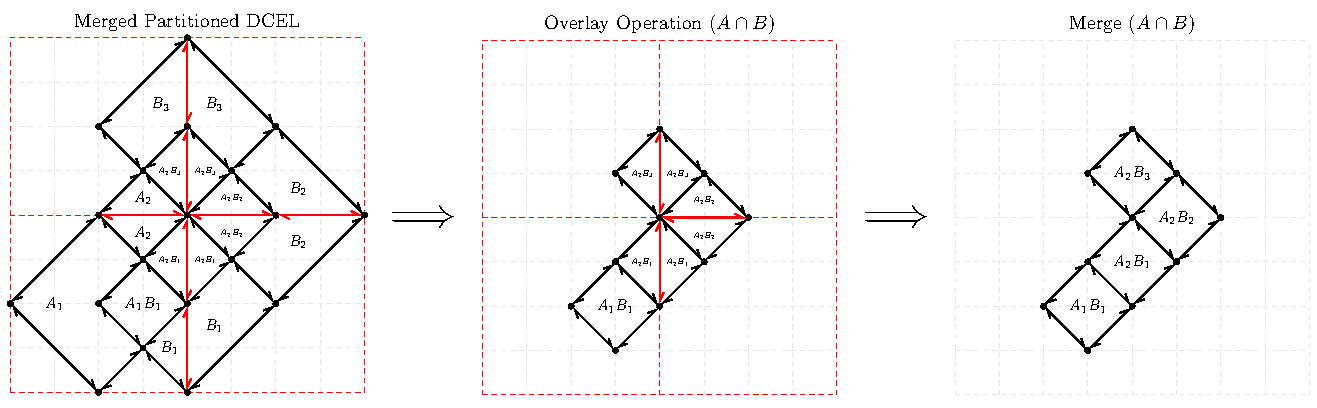
\includegraphics[width=\linewidth]{figures/03-OverlayParted2}
    \caption{Example of an overlay operation querying the distributed DCEL.} \label{fig:overlay_parted2}
\end{figure}

Figure \ref{fig:overlay_operations} shows the results of the five overlay operations supported by the scalable DCEL.  To obtain the results we query locally the DCEL filtering the faces according to the characteristics of its label.  For intersection ($A \cap B$), it filters just faces where its label contains both letters (A and B); On the other hand, for symmetric difference ($A \bigtriangleup B$), it filters faces where its labels contains just one of the letters (A or B).  For the case of difference between the layers ($A \setminus B$ or $B \setminus A$), it filters faces and labels according to the requested letter (either A or B). In the case of union ($A \cup B$), all the faces are retrieved. 

\begin{figure*}[!ht]
    \centering
    \tikzset{    
    node1/.style={
        above right
    }
}
\scalebox{0.5}{
    \begin{tikzpicture}
        \node[node1,label={$A \cup B$}]           at (0,0)  {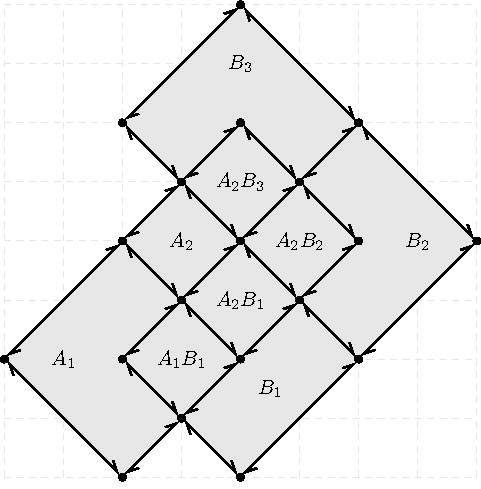
\includegraphics[scale=0.75]{figures/04/DCELUnion}};
        \node[node1,label={$A \cap B$}]           at (7,0)  {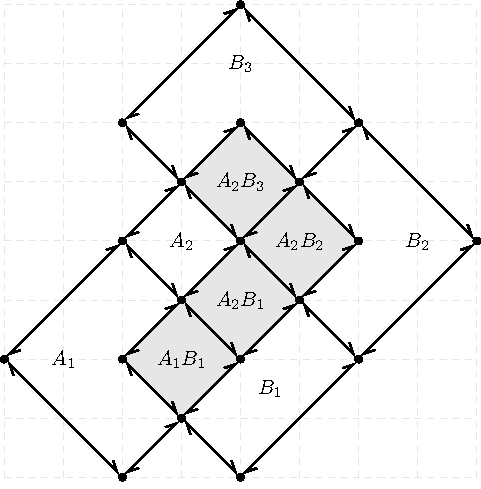
\includegraphics[scale=0.75]{figures/04/DCELIntersection}};
        \node[node1,label={$A \setminus B$}]      at (14,0) {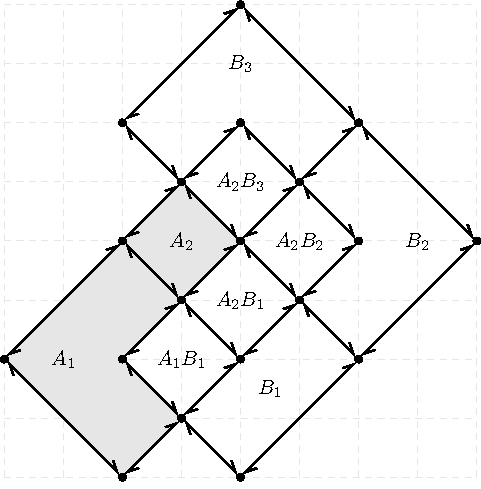
\includegraphics[scale=0.75]{figures/04/DCELDiffA}};
        \node[node1,label={$B \setminus A$}]      at (21,0) {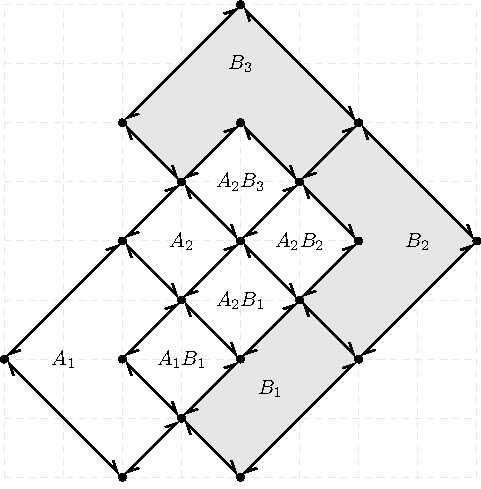
\includegraphics[scale=0.75]{figures/04/DCELDiffB}};
        \node[node1,label={$A \bigtriangleup B$}] at (28,0) {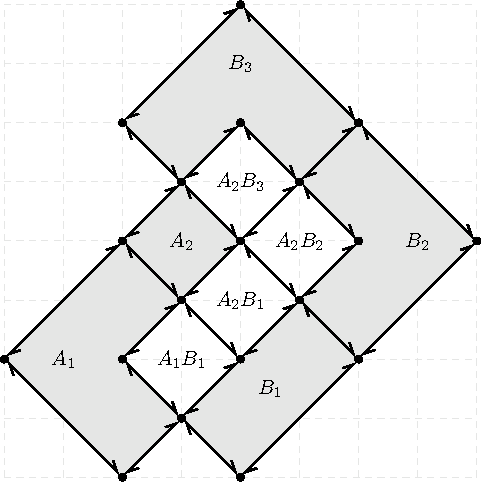
\includegraphics[scale=0.75]{figures/04/DCELDiff}};
    \end{tikzpicture}
}
    \caption{Results of the overlay operations supported by the scalable DCEL.}\label{fig:overlay_operations}
\end{figure*}

\subsection{Parallel DCEL Computation}
In this section explain:

* how the edges from the polygons are partitioned
* how to integrated the intersection of the edges and the boundary of the cells at partition time
* extract the edges which are connected and are fully contained by the cell, they can be reported directly.
* extract the edges which are connected but remains open because their are cut by the border of the cell.
* identify those edges which intersect the boundary and used to create new edges in the borders of the cell.  
* run the a variation of the sequential algorithm to connect the open edges and the edges from the borders of the cell.

prepare some graphics to explain the steps


\subsection{Cell inside polygon problem} \label{sec:anomalies}
The main goal of the proposal is to be able to divide the problem into smalls partitions for efficient processing.  Each partition collects the needed data and it is able to build its local DCEL without the need of query other partitions.  However, under this partition strategy, a new problem arises.  It happens when the partition schema (i.e. a quadtree) deliver a cell where no edges for any of the input layers are located.  The problem is even more complicated when a just hole in located inside a cell (figure \ref{fig:emptycells}).  The problem is that the empty cell (or the empty portion in the case of holes) has no access to which polygon it belongs making its corresponding labeling impossible.  

\begin{figure}[!ht]
    \centering
    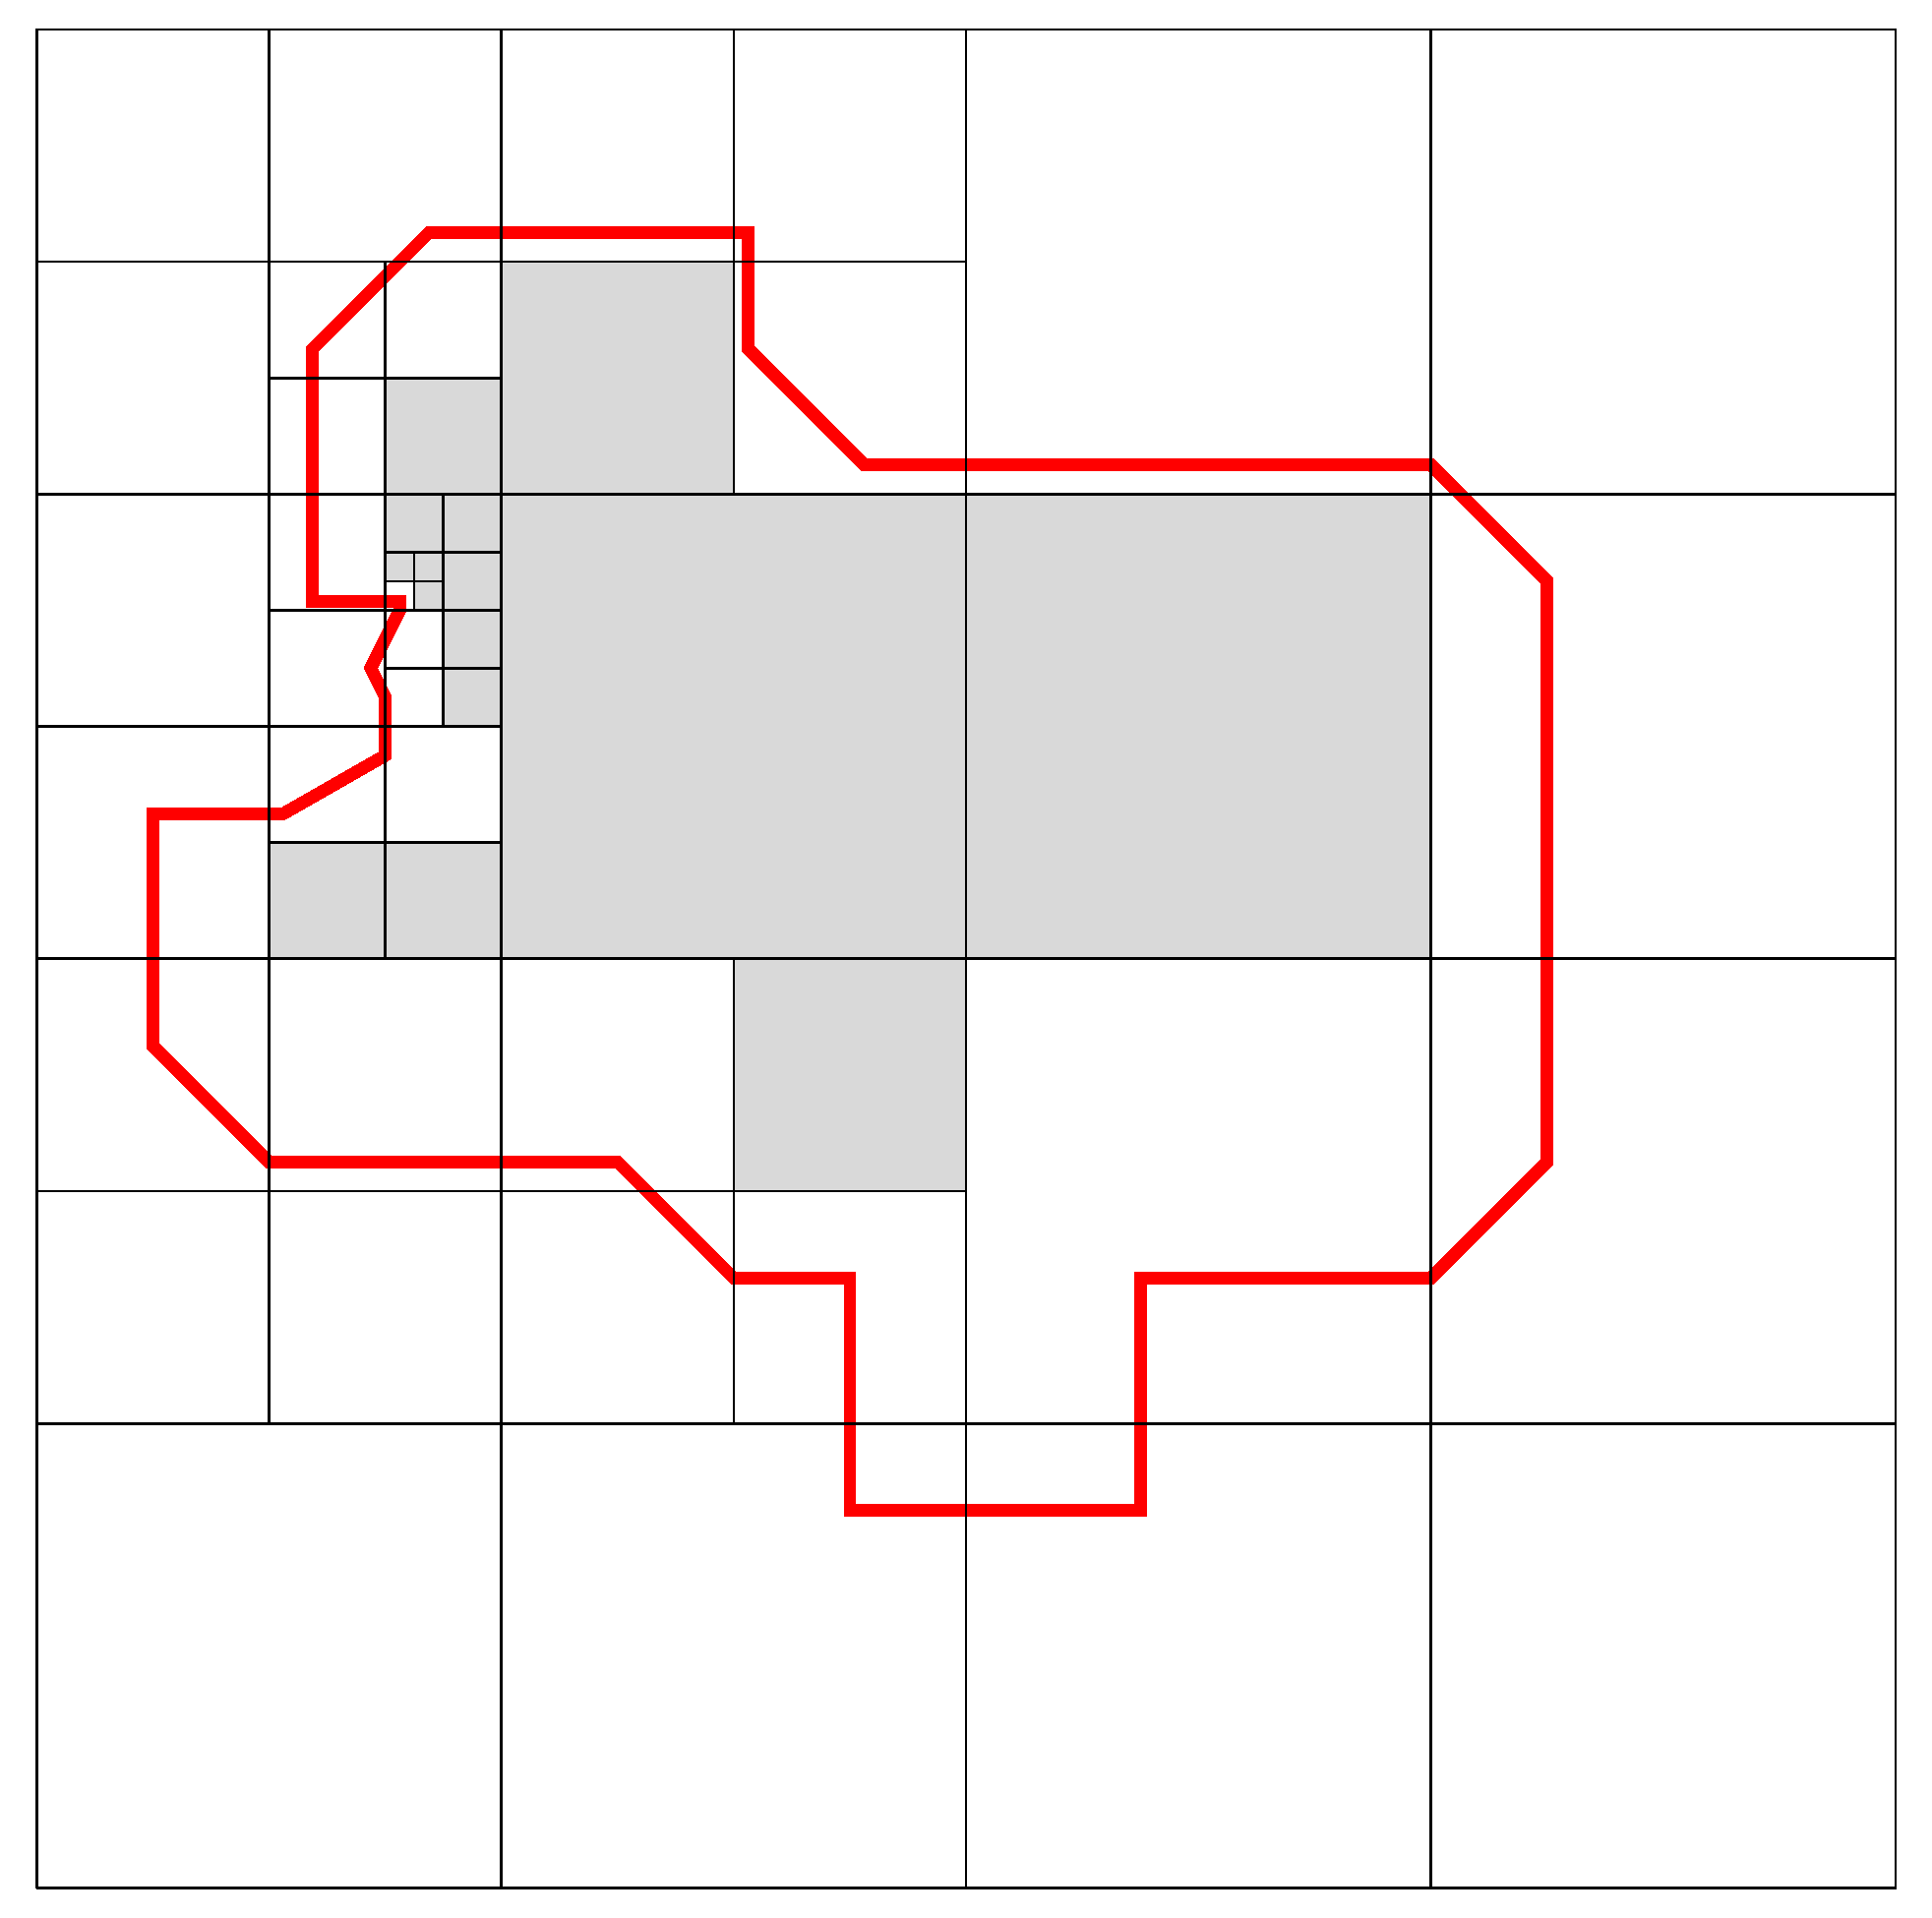
\includegraphics[page=1, width=0.4\textwidth]{figures/cellinpolygon/emptycells.pdf}
    \includegraphics[page=2, width=0.4\textwidth]{figures/cellinpolygon/emptycells.pdf}
    \caption{Example of empty cell and empty cell with holes cases.}\label{fig:emptycells}
\end{figure}

To solve the problem, an algorithm is proposed to find the next cell in the valid information about the polygon they are contained.  It is based on the branch information of the cell inside of the spatial index structure used during partition, also know as lineage (see figure \ref{fig:lineage_example} for an example).  For the sack of explanation, we will assume we use a quadtree, but the proposal could be easily adapted to other data structures such as grids.

After the partitioning strategy, a set of the cells is available with the following information: an unique cell identifier (id); a lineage, a string which provides the position and depth of the cell into the spatial index; and an envelope which is a polygon representation (a rectangle) of the boundaries of the cell.

The key of the proposal is to identify the centroid of the parent cell from the empty cell in question.  That point will allow us to retrieve the neighbour cells which can easily be queried if they have edges to extract the needed polygon information.  If all of them are still empty, we proceed to choose that one with the deepest level and recursively repeat the process.  Eventually, a non-empty cell will emerge and all the involved empty cells can be updated.  Figure \ref{fig:emptycellexample} shows a three iteration run of the algorithm with the example of figure \ref{fig:emptycells}.

\begin{figure}[!ht]
    \centering
    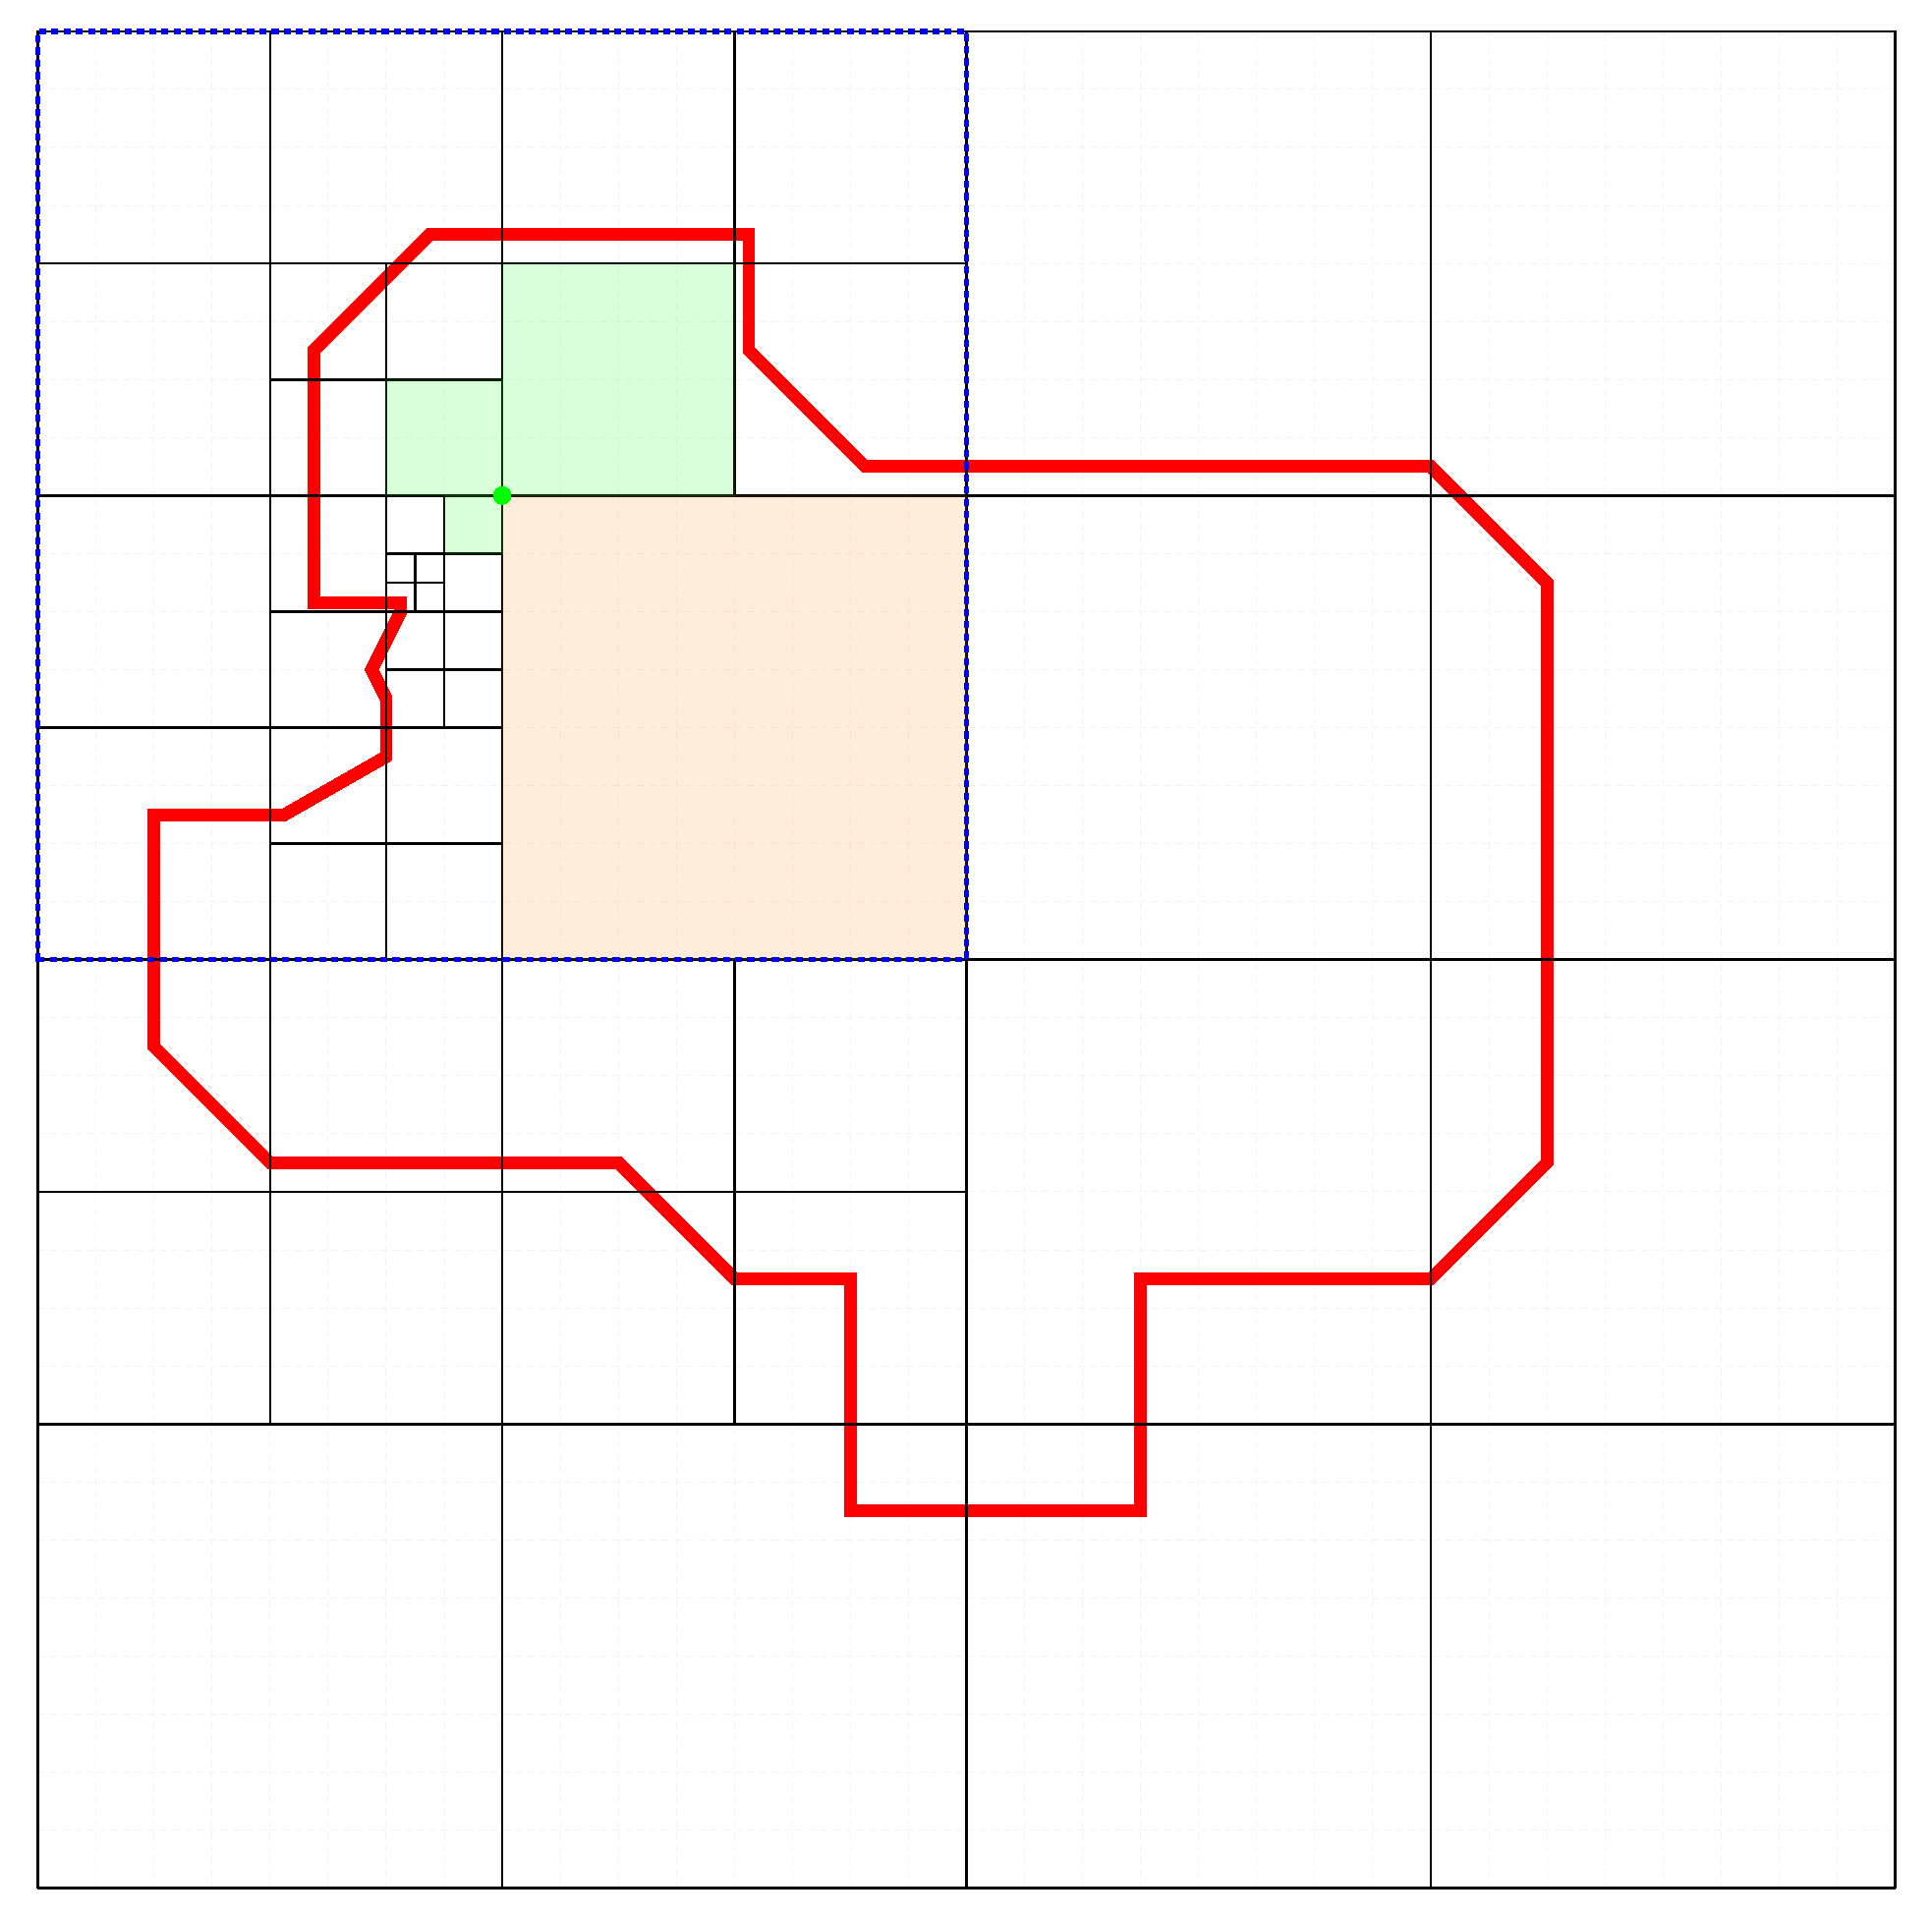
\includegraphics[page=1, width=0.49\linewidth]{figures/cellinpolygon/example}
    \includegraphics[page=2, width=0.49\linewidth]{figures/cellinpolygon/example}
    \includegraphics[page=3, width=0.49\linewidth]{figures/cellinpolygon/example}
    \caption{Three iterations of the proposed algorithm to find the next cell with valid edges from a empty cell.} \label{fig:emptycellexample}
\end{figure}

The details and pseudo code of the algorithm can be seen at appendix \ref{app:emptycells}.  We based of proposal in the following lemma and used it to proved our point with the subsequent proof.

\begin{lemma}
Four cells at the same level can not be empty.  At least one of them must have edges in order to force the split.
\end{lemma}

\begin{proof}
The $\textsc{getCellsInCorner}$ function will query the interior corner of a cell according to its position, that is the centroid of its cell parent.  The only cells which can intersect that point are cells at the same level of the current cell or their children.  If the 3 cells returned by $\textsc{getCellsInCorner}$ are empty, at least one of them must have a deeper level that the current cell.  Following that cell guarantees that the search space will be shrank at each iteration.  Eventually, the algorithm will reach the maximum level of the quadtree where all the involved cells will have the same level and, therefore, at least one of them must have edges.
\end{proof}

\subsection{Distributed overlay operators} \label{sec:overlay}
Once the distributed DCEL is ready for analysis, we have to take care on how it should be queried in order to take advantage of such distribution.  Section \ref{sec:strategy} shows the initial strategy to partition the study area and how each partition holds a section of the DCEL clipped to the cell boundary of that partition.  It is straightforward that we could query locally each of the sections but, once it is done, we should unify the results among contiguous partitions.

Faces in the interior of a partition (those which do not touch the boundary) are safe to be reported.  However, for those faces which share a half-edge with the boundary, there is a high chance that another section of that face is present in a contiguous partition and has to be checked.  

We execute a merging stage on the set of faces which touch the boundaries of each partition.  It performs a reduce operation pairing faces with the same label and dissolving their geometries.  For example, in figure \ref{fig:overlay_parted2}, it can be seen how faces in different partitions but with the same label are merged into final results by removing their common half-edges. 

\newpage
\section{Experiments}

\subsection{Real datasets}
In order to test our implementation, we used three datasets of polygons.  The first one is the California Census Tracts - CCT. The layer A collects the census tracts in California during 2000 meanwhile the layers B collects those ones for 2010.  Something to note with this dataset is that the differences between the layers no just show the changes in time but also they present a small spatial gap (due to technical reasons) between the polygons which will increase considerably the number of intersections and new faces the DCEL should be able to identify.

The second dataset is the complete Census Tracts dataset for all the states of the Union in mainland.  It was collected from the official website of the United States Census Bureau\footnote{\url{https://www2.census.gov/geo/tiger/TIGER2010/TRACT/}}.  The data was clipped to select just the states inside the continent to keep the study area as compact as possible and remove some territories that does not have complete data. The layers correspond to years 2000 and 2010. The two layers are quite similar although they also present a spatial gap similar than the CCT dataset.  The CCT dataset is a subset of this dataset just for the state of California.

The third dataset is from the Global Administration Areas - GADM\footnote{\url{https://gadm.org/}}. It collects geographical boundaries of the countries and their administrative divisions around the globe.  For the tests, we select the levels 2 (States) and level 3 (Counties).  However no all the countries show administrative level for counties, for that reason both layers shows similar number of polygons and edges. We take individual polygons, it is, any multi-polygon was divided and each polygon was manage independently. The details of the real datasets are summarized in table \ref{tab:datasets}.  Experiments runs on a cluster of 12 nodes running Apache Spark 2.4.  Each node has 9 cores and 12G memory available.

\begin{table}[!ht]
    \caption{Datasets details.}
    \label{tab:datasets}
    \begin{tabular}{c c c c}
        \toprule
        Dataset & Layer & Number        & Number    \\
                &       & of polygons   & of edges  \\
        \midrule
        CCT   & Polygons for 2000 & 7028 & 2711639  \\
              & Polygons for 2010 & 8047 & 2917450 \\
        MainUS& Polygons for 2000 & 64983 & 35417146  \\
              & Polygons for 2010 & 72521 & 36764043 \\
        GADM  & Polygons for Level 0 & 116995 & 32789444 \\
              & Polygons for Level 1 & 117891 & 37690256 \\
        \bottomrule
    \end{tabular}
\end{table}

\subsection{CCT dataset}

The first set of experiments aim to compare the performance of the SDCEL implementation over the CCT Dataset varying the number of partitions used to divide the data. It sets the parameters of the quadtree used to split the data to obtains different values from coarse (100) to fine (15K) number of partitions (left part in figure \ref{fig:ca}).  Clearly there are a trade-off in this case.  The more partitions, each subdivision will have to deal with a smaller number of edges will means a faster execution.  However, if the number of partitions is too high, the cost to divide and collect the results will have an impact.  We can see that an optimal value can be reached around 7K partitions.  A zoom of this part of the plot is shown in figure \ref{fig:ca}.

In addition with the partition analysis, we compare the performance of the SDCEL implementation against the sequential solution offered by the CGAL library.  The independent column in the right of figure \ref{fig:ca} shows its execution time.  Clearly, the appropriate setting for the number of partitions of SDCEL can beat the sequential implementation by several orders of magnitude.

\begin{figure}[!ht]
    \centering
    \subfloat[SDCEL vs CGAL. \label{fig:ca_a}]{%
        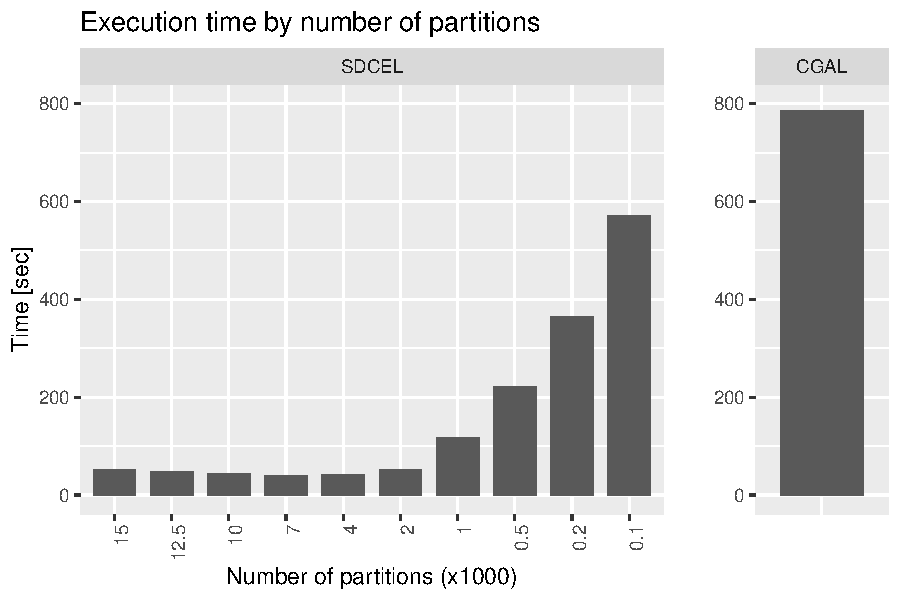
\includegraphics[width=0.9\linewidth]{figures/experiments/CA/CA.pdf}
    } \\
    \subfloat[Focus on the most relevant number of partitions. \label{fig:ca_b}]{%
        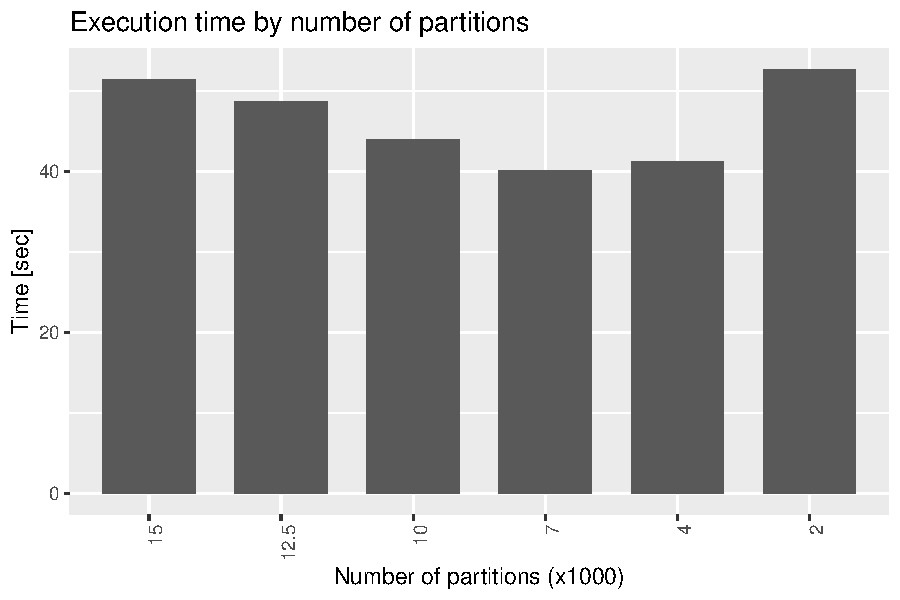
\includegraphics[width=0.9\linewidth]{figures/experiments/CA/CA_sample.pdf}
    }
    \caption{Experiments with CCTAL dataset.} \label{fig:ca}
    \Description[Experiments with the CCTAL dataset]{This figure shows the experiments using the CCTAL dataset.}
\end{figure}

\subsection{MainUS and GADM datasets}

\begin{figure}[!ht]
    \centering
    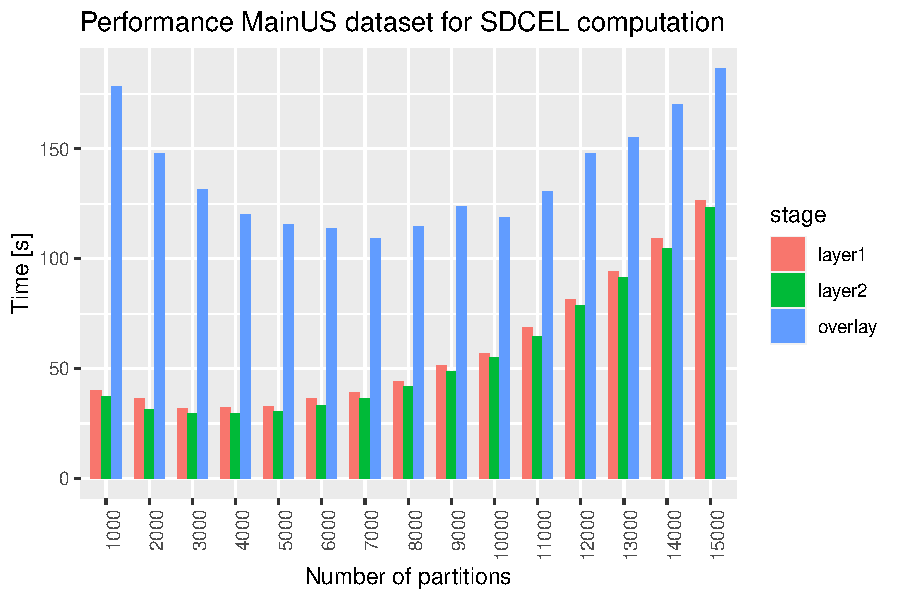
\includegraphics[width=\linewidth]{figures/experiments/MainUS/MainUS.pdf}
    \caption{Performance with MainUS dataset.} \label{fig:mainus}
    \Description[Experiments with the MainUS dataset]{This figure shows the experiments using the MainUS dataset.}
\end{figure}

\begin{figure}[!ht]
    \centering
    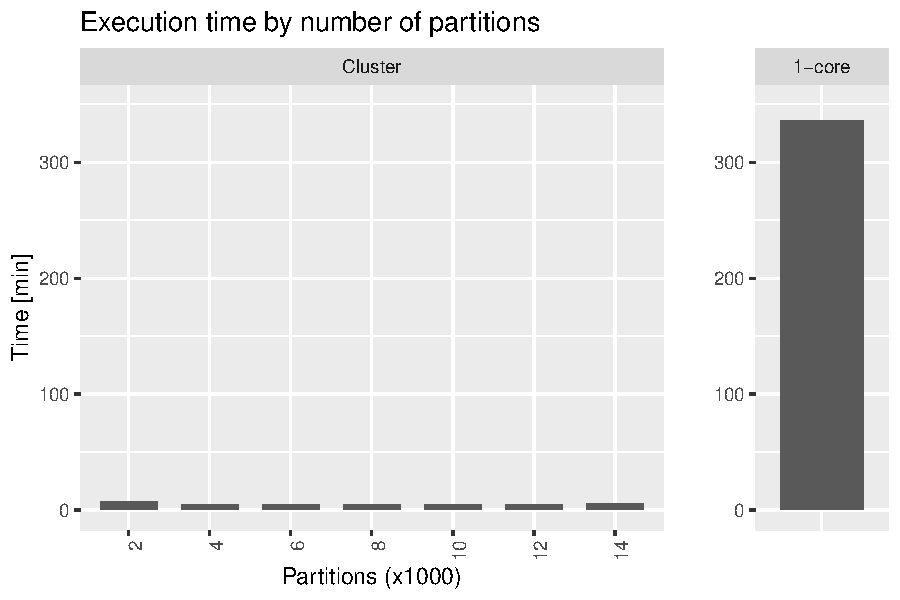
\includegraphics[width=\linewidth]{figures/experiments/GADM/GADM.pdf}
    \caption{Performance with GADM dataset.} \label{fig:gadm}
    \Description[Experiments with the GADM dataset]{This figure shows the experiments using the GADM dataset.}
\end{figure}

The CCT dataset is relatively small but useful in order to compare with the sequential alternative.  However, the CGAL library is unable to deal with big spatial data.  For MainUS and GADM datasets, we only present the results for SDCEL given that CGAL crashes when run this volume of data.  Figure \ref{fig:mainus} show the execution time of SDCEL varying the number of partitions and breaking down the execution time by stages.  Here, the time shows the performance to create the individual DCELs for each of the layers (labeled as layer1 and layer2) in addition to the time for the overlay of the two individual DCELs.  We can seen a similar trade-off as with CCT dataset in each of the stages.  We can identify a optimal number of partitions around the 6K -8K partitions.  

Figure \ref{fig:gadm} shows a similar experiment over the GADM dataset.  It plots the execution time for the SDCEL construction also divided by stages. We could identify a peak performance using between 12K and 16K partitions.  The characteristics of this dataset make it more sensible during the construction of individual DCELs particularly for the second layers which have more small polygons concentrated in some areas.

\subsection{Testing overlay alternatives}
In this section we evaluate the methods described in section \ref{sec:alternative_methods}.  We used the top 8 states from the MainUS dataset to evaluated the alternatives.  It measures the execution time of the overlay at the master/root node (`At master/root' tag), performing partitions by segment's label (`By label' tag) and performing an intermediate step at a given level (`At level [X]' tag, where X is the level given by the user).  Figure \ref{fig:overlay_tester} shows the results of the testing.  It clearly shows that the overlay by label partitions gives the best results in all the tests.

\begin{figure}[!ht]
    \centering
    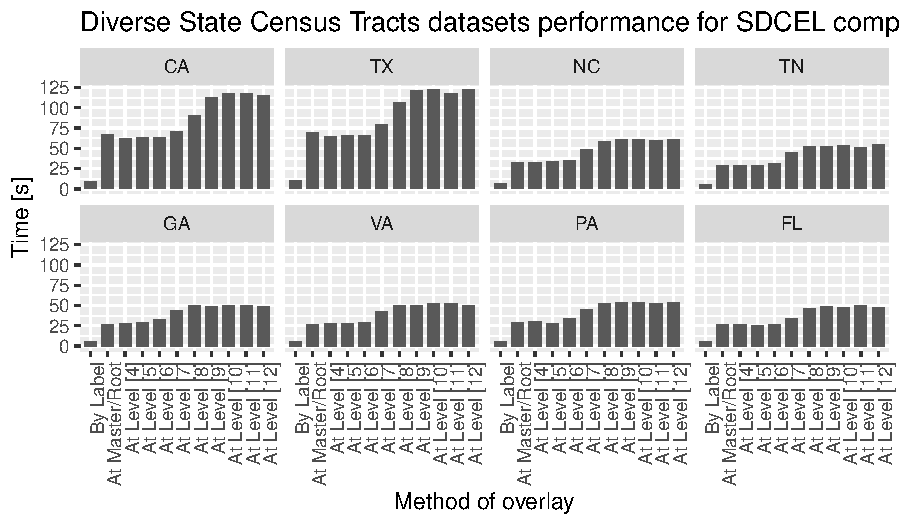
\includegraphics[width=\linewidth]{figures/experiments/Overlay_Tester/Overlay_Tester}
    \caption{Overlay methods evaluation.}\label{fig:overlay_tester}
    \Description[Overlay methods evaluation]{This figure shows the overlay methods evaluation.}
\end{figure}


\subsection{Speed up and scale up analysis}

Finally we analyze the scalability of the implementation through the speed up and scale up tests.  For the speed up, the GADM dataset was used with different amount of resources, in this case the number of available nodes.  Each time, the nodes were duplicated and the performance was measured.  Figure \ref{fig:gadm_speedup} shows  how as resources double, the response time is almost cut in half each time, as it is expected.

In the case of the scale up test, the workload was also modified.  The GADM dataset was split in 4 regions slightly similar in the number of edges they contain.  At each iteration, both the size of the data and the amount of available resources were doubled. As it was expected, the performance at each scenario should not change significantly as it is shown in figure \ref{fig:gadm_scaleup}.

\begin{figure}[!ht]
    \centering
    \subfloat[MainUS Speed Up \label{fig:mainus_speedup}]{%
        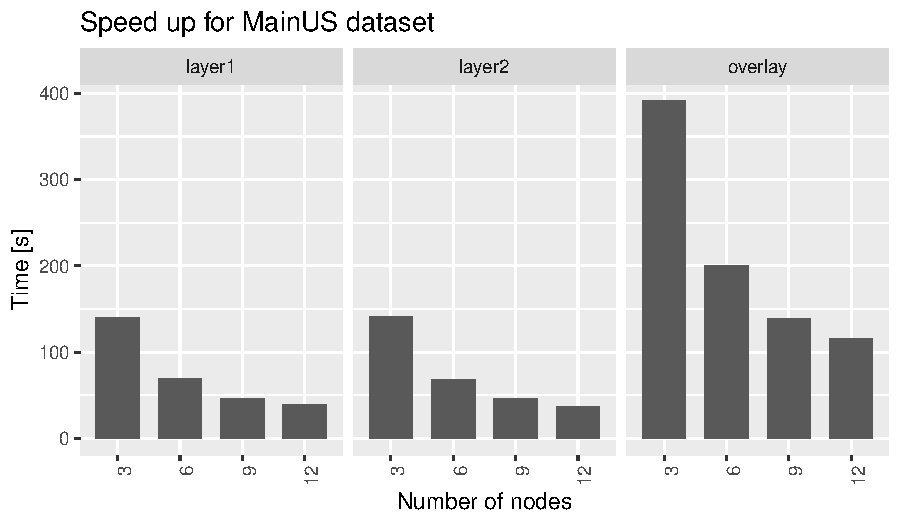
\includegraphics[width=0.9\linewidth]{figures/experiments/MainUS_speedup/MainUS_speedup}
    } \\
    \subfloat[MainUS Scale Up \label{fig:mainus_scaleup}]{%
        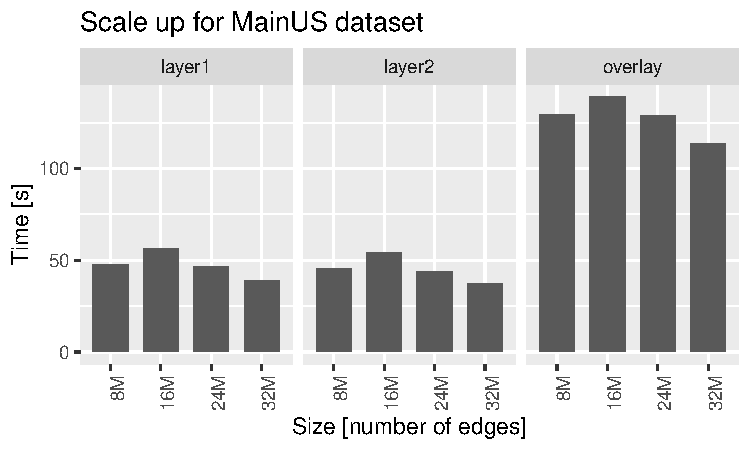
\includegraphics[width=0.9\linewidth]{figures/experiments/MainUS_scaleup/MainUS_scaleup}
    }
    \caption{Speed Up and Scale Up experiments for MainUS dataset.} \label{fig:mainus_speed_scale}
    \Description[MainUS Speed Up and Scale Up experiments.]{This figure shows the experiments for speed up and scale up analysis for the MainUS dataset.}
\end{figure}

\begin{figure}[!ht]
    \centering
    \subfloat[GADM Speed Up \label{fig:gadm_speedup}]{%
        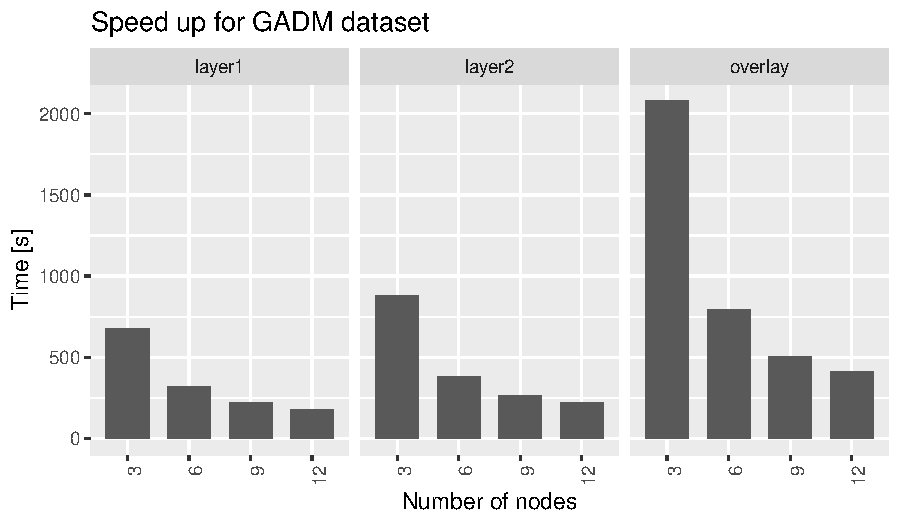
\includegraphics[width=0.9\linewidth]{figures/experiments/GADM_speedup/GADM_speedup}
    } \\
    \subfloat[GADM Scale Up \label{fig:gadm_scaleup}]{%
        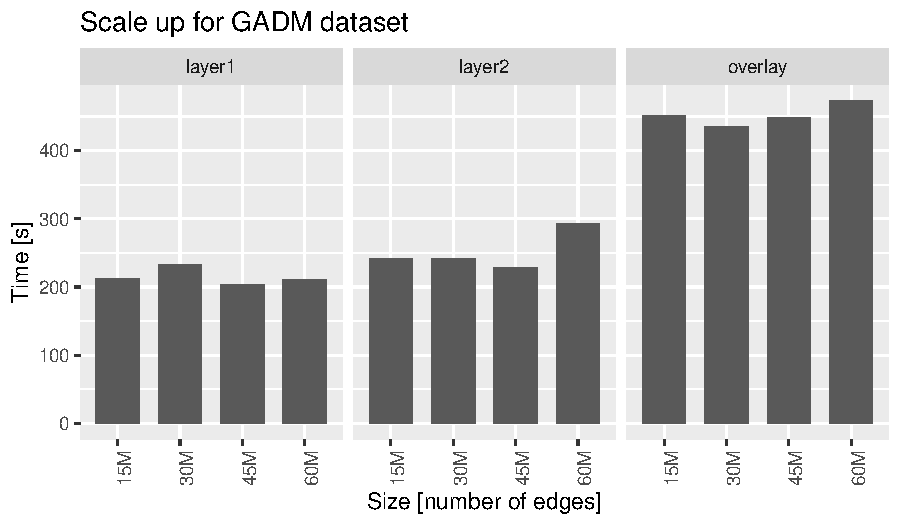
\includegraphics[width=0.9\linewidth]{figures/experiments/GADM_scaleup/GADM_scaleup}
    }
    \caption{Speed Up and Scale Up experiments for GADM dataset.} \label{fig:gadm_speed_scale}
    \Description[GADM Speed Up and Scale Up experiments.]{This figure shows the experiments for speed up and scale up analysis for GADM dataset.}
\end{figure}

\subsection{Unbalance cell analysis}

This section discusses the experiments and evaluation of the method of filter by sweep proposed in section \ref{sec:unbalance}. Figure \ref{fig:unbalance_tester1} shows the behaviour of the two methods (filter by sweep and traditional) under controlled data.  Edges from the state of Pennsylvania where taken increasing from one of the layers adding 3K edges each time and then an overlay over another layer of 3K was performed.  It simulates the actions inside an individual cell when an unbalanced number of edges for each layer must to be evaluated. It can be seen that once the data from the involved layers show increasingly unbalanced amount of data (that is, much more edges from one of the layers than the other) the filter by sweep method overcomes the traditional one on those cells with this kind of data.

\begin{figure}
    \centering
    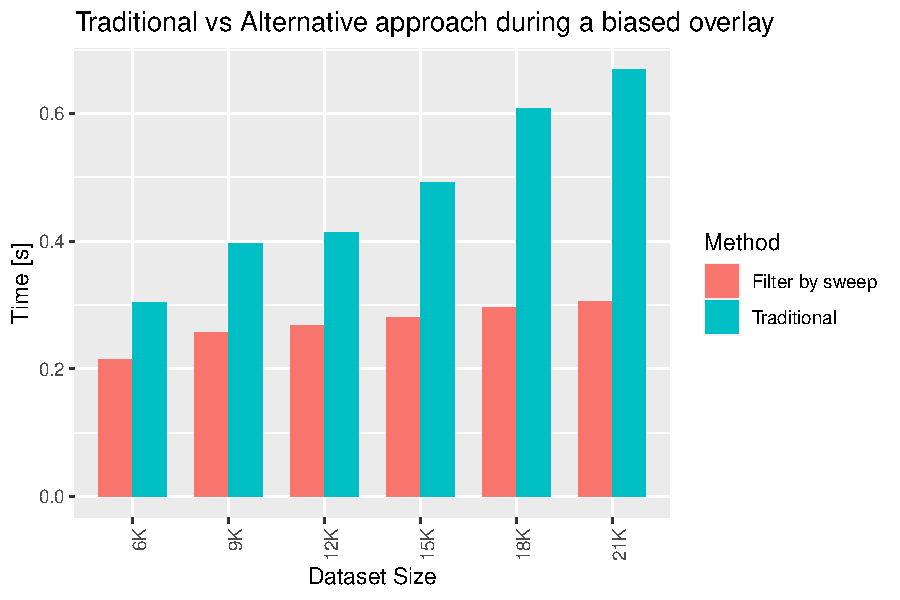
\includegraphics[width=\linewidth]{figures/experiments/Unbalance_Tester/Unbalance_Tester01.pdf}
    \caption{Unbalance cell methods evaluation.}\label{fig:unbalance_tester1}
    \Description[Unbalance cell methods evaluation]{This figure shows the Unbalance cell methods evaluation.}
\end{figure}

In addition, figure \ref{fig:unbalance_tester2} shows a similar scenario, this time using real data from the construction of the overlay DCEL of GADM dataset. For this experiment, a number of 10 cells were chosen with different percentage of disparity. It means that a 0.1 (10\%) difference happens when a layers is 10\% bigger than the other one. An average of the 10 cells for each case is shown in the figure and it compares the traditional method and the filter by sweep alternative.  Similar than in the previous case, it can be seen that the proposed method works better in cases where the number of edges for each layer is significant.

\begin{figure}
    \centering
    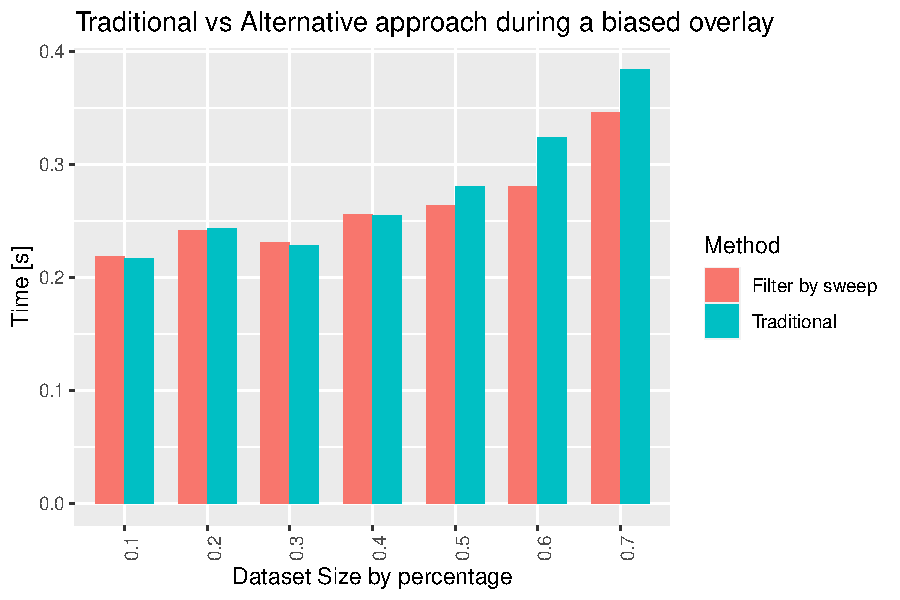
\includegraphics[width=\linewidth]{figures/experiments/Unbalance_Tester/Unbalance_Tester02.pdf}
    \caption{Unbalance cell methods evaluation.}\label{fig:unbalance_tester2}
    \Description[Unbalance cell methods evaluation]{This figure shows the Unbalance cell methods evaluation.}
\end{figure}

\bibliographystyle{IEEEtran}
\bibliography{sdcel.bib}

\section{Empty Cell Algorithm}\label{app:emptycells}
Algorithms \ref{alg:one} and \ref{alg:two} explains the steps to obtain a near quadtree cell which guarantee the presence of edges and how select the set of three cells around of a given corner respectively.  The latter is used to choose a possible path if the current cell is empty and it needs to identify at which polygon it belongs.  The former (using the latter) ensures the finding of a cell with the polygons' edges needed to determine the enclosing polygon.

\begin{algorithm}\caption{\textsc{getNextCellWithEdges} algorithm}\label{alg:one}
    \textbf{Require:} a quadtree with cell envelopes $\mathcal Q$ and map of cells and their edge count $\mathcal M$.
    \begin{algorithmic}[1]
    \Function{ getNextCellWithEdges }{ $\mathcal Q$, $\mathcal M$ }
        \State $\mathcal C \gets $ list of empty cells in $\mathcal M$
        \ForEach{ $emptyCell$ in $\mathcal C $ }
            \State initialize $cellList$ with $emptyCell$ 
            \State $nextCellWithEdges \gets null$
            \State $referenceCorner \gets null$
            \State $done \gets false$
            \While{ not $done$ } 
                \State $c \gets $ last cell in $cellList$ 
                \State $cells, corner \gets \textsc{getCellsAtCorner}(\mathcal Q, c)$ \Comment{ return 3 cells and the reference corner }
                \ForEach{$cell$ in $cells$}
                    \State $nedges \gets$ get edge count of $cell$ in $\mathcal M$ 
                    \If{ $nedges > 0$ }
                        \State $nextCellWithEdges \gets cell$
                        \State $referenceCorner \gets corner$
                        \State $done \gets true$
                    \Else
                        \State add $cell$ to $cellList$
                    \EndIf
                \EndFor
            \EndWhile
            \ForEach{ $cell$ in $cellList$ }
                \State \textbf{output}($cell$, \\
                \hspace{2.5cm} $nextCellWithEdges$, $referenceCorner$)
                \State remove $cell$ from $\mathcal C$
            \EndFor
        \EndFor
    \EndFunction
    \end{algorithmic}
\end{algorithm}

\begin{algorithm} \caption{\textsc{getCellsAtCorner} algorithm}\label{alg:two}
    \begin{algorithmic}
    \Require a quadtree with cell envelopes $\mathcal Q$ and a cell $c$.
    \Function{ getCellsInCorner }{ $\mathcal Q$, $c$ }
        \State $region \gets $ last character in $c.lineage$
        \Switch{ $region$ }
            \Case{ `0' }
                \State $corner \gets$ left bottom corner of $c.envelope$
            \EndCase
            \Case{ `1' }
                \State $corner \gets$ right bottom corner of $c.envelope$
            \EndCase
            \Case{ `2' }
                \State $corner \gets$ left upper corner of $c.envelope$
            \EndCase
            \Case{ `3' }
                \State $corner \gets$ right upper corner of $c.envelope$
            \EndCase
        \EndSwitch
        \State $cells \gets$ cells which intersect $corner$ in $\mathcal Q$
        \State $cells \gets cells - c$ \Comment{ Remove the current cell from the intersected cells }
        \State $cells \gets$ sort $cells$ on basis of their depth \Comment{ using $cell.lineage$ }
        \State \Return{ ($cells$, $corner$) }
    \EndFunction
    \end{algorithmic}
\end{algorithm}

\begin{figure}
    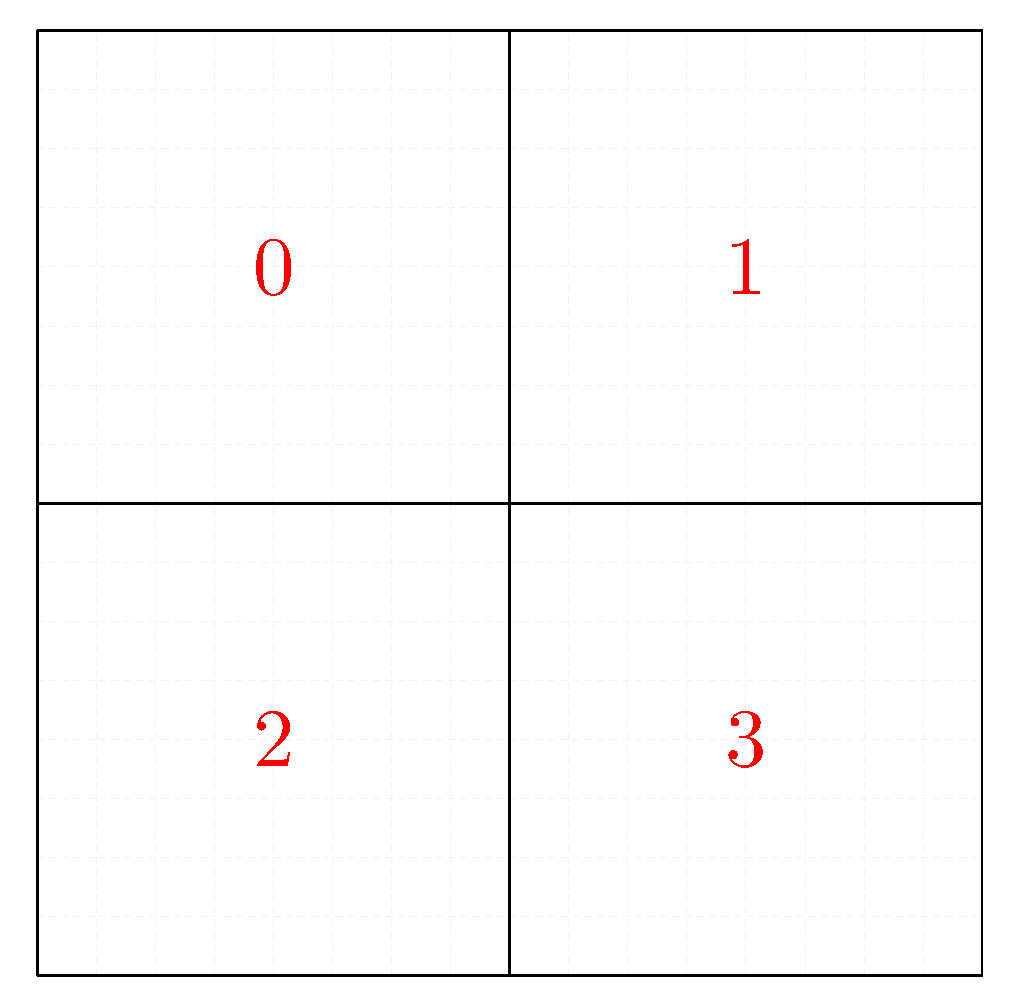
\includegraphics[page=1,width=0.32\linewidth]{figures/cellinpolygon/lineage}
    \includegraphics[page=2,width=0.32\linewidth]{figures/cellinpolygon/lineage}
    \includegraphics[page=3,width=0.32\linewidth]{figures/cellinpolygon/lineage}
    \caption{Lineage can provide the cell's position (string's last character) and its depth (string's length).}
    \label{fig:lineage_example}
    \Description[Lineage example]{Lineage can provide the cell's position (string's last character) and its depth (string's length).}
\end{figure}

\section{Lineage example}
See figure \ref{fig:lineage_example} for an illustration of the lineage used in a quadtree.


\end{document}
